\section{MAB Objective}
The objective of the agent, as stated earlier is to find the best arm with the maximum expected reward, and keep pulling it to obtain maximum reward.
In a more formal notation, one could say, that we want to estimate $Q(a_i)$ and maximize it, $Q(a^*_i) = \max_i{Q(a_i)}$

\begin{itemize}
    \item Let, $r_{i,k}$ be the reward sample acquired when $i^{th}$ arm is selected for the $k^{th}$ time.
    \item Define:
    \begin{equation*}
        \begin{split}
            Q(a_i) &= \frac{\sum_k r_{i,k}}{\sum_{k:r_{i,k}}\mathbf{1}}\\
            Q_{k+1}(a_i) &= Q_k(a_i) + \alpha ( r_{i,k} - Q_k(a_i))\\
            Q(a^*_i) &= \text{max}_i \{Q(a_i)\}
        \end{split}
    \end{equation*}
    \item Setting $\alpha = \frac{1}{k_i + 1}$ yields the average.
\end{itemize}

\subsection{Epsilon-Greedy}
Epsilon-Greedy ($\varepsilon$-greedy) is the most common and simplest algorithm for balancing the trade-off between exploring and exploiting by choosing them randomly.
\begin{itemize}
    \item The $\epsilon$-greedy strategy selects arm $a^* = \text{argmax}_i \{Q_k(a_i)\}$ with a probability of $1-\epsilon$ and selects any arbitrary arm with a probability $\epsilon$.
\end{itemize}
Assume that we explore $n$ options at the initial stage.
Then, by the $\varepsilon$-greedy algorithm, (1-$\varepsilon$) percent time we greedily exploit the best option $k$ among the $n$ options, and during the remaining $\epsilon$ percent time other options are randomly explored for a better decision than the previously best option $k$.
The value of $\varepsilon$ is set to 10\% generally.

\subsubsection{Epsilon Decreasing Method}
Epsilon deceasing is similar to the $\varepsilon$-greedy method.
The $\varepsilon$ in the $\varepsilon$-greedy method is remained \texttt{fixed}, while in the epsilon decreasing method the $\varepsilon$ value gradually \textit{decreases} over time.
The number of exploring new options gradually \textit{decreases} with the \textit{decrease} of the value $\varepsilon$ and meaning that the best option becomes more certain in the process.


\subsection{Softmax}
Although $\epsilon$-greedy action selection is an effective and popular means of balancing exploration and exploitation in RL, one drawback is that when it explores it chooses equally among all actions.
This means that it is as likely to choose the worst appearing action as it is to choose the next-to-best action.
In situations where this is not an expected exploratory step, this can produce unsatisfactory results.
But these can be mitigated by:
\begin{itemize}
    \item An obvious solution is to vary the action probabilities as a graded function of estimated value.
    \item The greedy action is still given the highest selection probability, but all the others are ranked and weighted according to their value estimates.
\end{itemize}
These are called \textbf{softmax} action selection rules.

\begin{itemize}
    \item The Softmax Algorithm selects arms with a probability proportional to the current value estimates, i.e.
    $$\pi_k (a_i) = \frac{\exp{(Q_k(a_i)/\tau)}}{\sum_j \exp{(Q_k(a_j)} / \tau)}$$
\end{itemize}
where $\tau$ is a positive parameter called the \textbf{Temperature}.
\begin{itemize}
    \item High temperatures cause the actions to be (nearly) \textit{equiprobable}, i.e. it behaves like a random function.
    \item Low temperatures cause a greater difference in selection probability for actions that differ in their estimates.
    \item In the limit $\tau \rightarrow 0$, softmax action selection becomes the same as \textit{Greedy Action} Selection.
\end{itemize}
Of course, the Softmax effect can be produced in a large number of ways other than by a \textbf{Gibbs Distribution}.

\noindent Asymptotic Convergence is Guaranteed. 

\subsection{Regret Optimality}
Maximizing the total rewards obtained, by minimizing the regret while learning.
\begin{figure}[h]
    \centering
    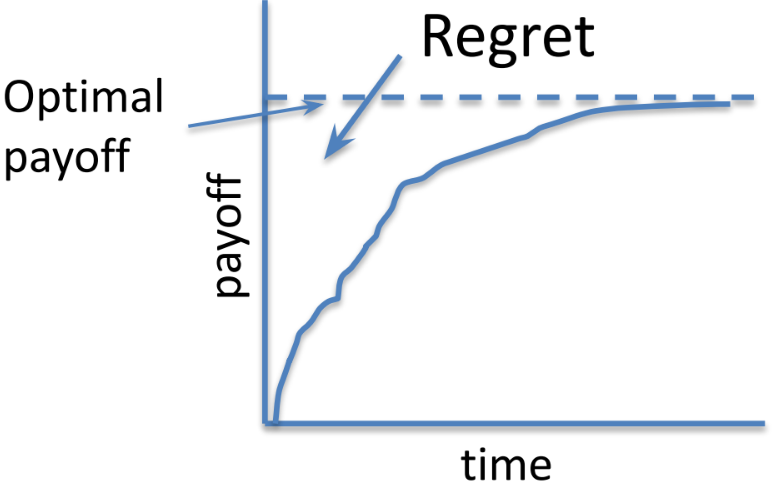
\includegraphics[width=0.6\linewidth]{resources/img/Regret_Optim_01.png}
    \caption{Regret}
    \label{fig:Regret}
\end{figure}

\subsection{PAC Optimality Frameworks}
\textbf{Probably Approximately Correct (PAC)} frameworks are usually used for identification of an $\epsilon$-optimal arm with probability $1-\delta$.

\noindent It is also $\epsilon$-optimal, meaning that, it satisfies the Mean of the selected arm.

\noindent Minimizes the Sample Complexity, i.e. the order of samples required for such an arm identification.

\section{Upper Confidence Bounds (UCB)}

\begin{minipage}{0.85\textwidth}
\begin{itemize}[leftmargin=*]
    \item Here, the arm with the best estimate $r^*$ so far serves as a benchmark, and other arms are played only if the upper bound of a suitable confidence interval is at least $r^*$.
    \item Simplest Approach --- Be Greedy with respect to UCBs.
    \item The Sub-optimal arm $j$ (say) is played fewer than $((8/\Delta_j) \ln n)$ times. 
    \item Further improvements on the base UCB Algorithm, called \texttt{UCB1}, focused mostly on reducing the constants.
    \item \texttt{UCB1} algo states that:\\
    \textbf{Loop: Until Convergence}\\
        \hspace{20pt} --- Play machine $j$ that maximizes $$\bar{x_j} + \sqrt{\frac{2 \ln n}{n_j}},$$ where $\bar{x_j}$ is the average reward obtained from machine $j$, $n_j$ is the number of times machine $j$ has been played so far, and $n$ is the overall (or total) number of plays done so far (including all arms).
\end{itemize}
\end{minipage}%
\hfill
\begin{minipage}{0.15\textwidth}
    % \centering
    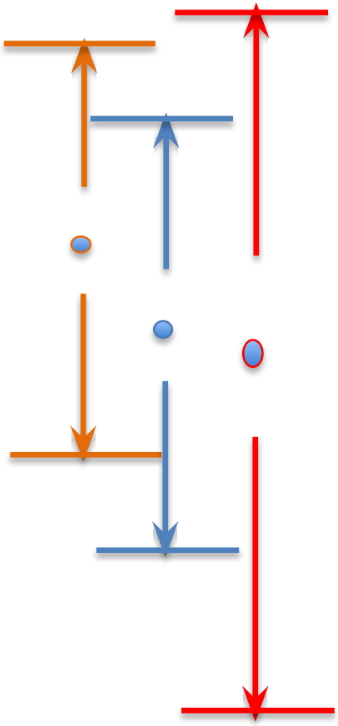
\includegraphics[width=\textwidth]{ucb_01.png}
\end{minipage}%
